\chapter{Statistical Testing of GP-EKF}
Inspired by \cite{hexeberg}, we will test the performance of the model for straight-line trajectoires and curved trajectories independently.
\section{Straigth-line trajectories}
We use the first $100$ randomly sampled trajectories satisfying the following requirements:
\begin{enumerate}
    \item The sum of subsequent changes in \acrshort{cog} must be less than $30$ degrees, i.e. the trajectory must be close to a straight line.
    \item There must be sufficient data available for training in the neighbourhood around the initial starting point, with similar initial heading and speed.
\end{enumerate}
\subsection{Prediction Errors}
Insert quantile or box plot here
\subsection{Consistency}
Insert plot of NEES here

\section{Curved Trajectories}
We use the first $100$ randomly sampled trajectories satisfying the following requirements:
\begin{enumerate}
    \item The sum of subsequent changes in \acrshort{cog} must be greater than $40$ degrees, i.e., the trajectory must be close to a straight line.
    \item There must be sufficient data available for training in the neighborhood around the initial starting point, with similar initial heading and speed.
\end{enumerate}

\subsection{Trajectory Error}
The trajectory error is found by comparing the predicted position with the ground truth. As the predicted trajectory is simulated in discrete time, the points with closest timestamps are used for comparison. With $\Delta T = 10\text{ seconds}$, the maximum error in time is $\frac{\Delta T}{2} = 5 \text{ seconds}$, which is considered to be acceptable considering the time-horizon of between $15$ and $30$ minutes. Mean and median summary statistics for the trajectory errors is shown in \cref{table:stats_curved_trajectory_error}.
\begin{table}[h]
    \begin{subtable}{\textwidth}
        \makebox[\textwidth][c]{
            \begin{tabular}{llrrrrr}
                \toprule
                               & Time [Minutes]    & 5    & 10   & 15   & 20   & 25    \\
                Method         & Training Source   &      &      &      &      &       \\
                \midrule
                CVM            & COG/SOG from AIS  & 1451 & 3492 & 6354 & 9925 & 17156 \\
                GP-EKF         & COG/SOG from AIS  & 806  & 1674 & 2437 & 2838 & 3879  \\
                               & Finite Difference & 656  & 1356 & 1850 & 2273 & 2371  \\
                GP-EKF w/ PDAF & COG/SOG from AIS  & 749  & 1532 & 2165 & 2358 & 3003  \\
                               & Finite Difference & 664  & 1312 & 1776 & 2166 & 2240  \\
                \bottomrule
            \end{tabular}
        }
        \caption{Mean Error}
    \end{subtable}
    \begin{subtable}{\textwidth}
        \makebox[\textwidth][c]{
            \begin{tabular}{llrrrrr}
                \toprule
                               & Time [Minutes]    & 5   & 10   & 15   & 20   & 25    \\
                Method         & Training Source   &     &      &      &      &       \\
                \midrule
                CVM            & COG/SOG from AIS  & 952 & 2515 & 4828 & 8597 & 14719 \\
                GP-EKF         & COG/SOG from AIS  & 648 & 1311 & 1931 & 2412 & 3275  \\
                               & Finite Difference & 457 & 931  & 1369 & 1873 & 1784  \\
                GP-EKF w/ PDAF & COG/SOG from AIS  & 574 & 1117 & 1513 & 1697 & 2016  \\
                               & Finite Difference & 480 & 881  & 1323 & 1719 & 1654  \\
                \bottomrule
            \end{tabular}
        }
        \caption{Median Error}
    \end{subtable}
    \caption{Mean and Median trajectory error for $350$ random predictions.}
    \label{table:stats_curved_trajectory_error}
\end{table}

\subsection{Path Error}
The path error is defined to be the closest point in the predicted trajectory to each point in ground-truth, under the constraint that the corresponding predicted timestamps must be monotonically increasing. In other words, the path cannot move backwards in time. The results are summarized in \cref{table:stats_curved_trajectory_path_err}.
\begin{table}[h]
    \begin{subtable}{\textwidth}
        \makebox[\textwidth][c]{
            \begin{tabular}{llrrrrr}
                \toprule
                               & Time [Minutes]    & 5   & 10   & 15   & 20   & 25   \\
                Method         & Training Source   &     &      &      &      &      \\
                \midrule
                CVM            & COG/SOG from AIS  & 562 & 1458 & 2929 & 4149 & 6466 \\
                GP-EKF         & COG/SOG from AIS  & 312 & 737  & 1465 & 1986 & 3010 \\
                               & Finite Difference & 369 & 605  & 747  & 730  & 605  \\
                GP-EKF w/ PDAF & COG/SOG from AIS  & 285 & 616  & 1190 & 1485 & 2172 \\
                               & Finite Difference & 366 & 569  & 693  & 687  & 593  \\
                \bottomrule
            \end{tabular}
        }
        \caption{Mean}
    \end{subtable}
    \begin{subtable}{\textwidth}
        \makebox[\textwidth][c]{
            \begin{tabular}{llrrrrr}
                \toprule
                               & Time [Minutes]    & 5   & 10  & 15   & 20   & 25   \\
                Method         & Training Source   &     &     &      &      &      \\
                \midrule
                CVM            & COG/SOG from AIS  & 188 & 856 & 1967 & 3405 & 5524 \\
                GP-EKF         & COG/SOG from AIS  & 141 & 328 & 982  & 1388 & 2621 \\
                               & Finite Difference & 203 & 398 & 447  & 435  & 376  \\
                GP-EKF w/ PDAF & COG/SOG from AIS  & 133 & 248 & 643  & 866  & 1347 \\
                               & Finite Difference & 220 & 393 & 429  & 405  & 373  \\
                \bottomrule
            \end{tabular}
        }
        \caption{Median}
    \end{subtable}
    \caption{Mean and Median path error for $350$ curved trajectory predictions.}
    \label{table:stats_curved_trajectory_path_err}
\end{table}

\section{Comparing GP-EKF to CVM}
\begin{figure}[h]
    \centering
    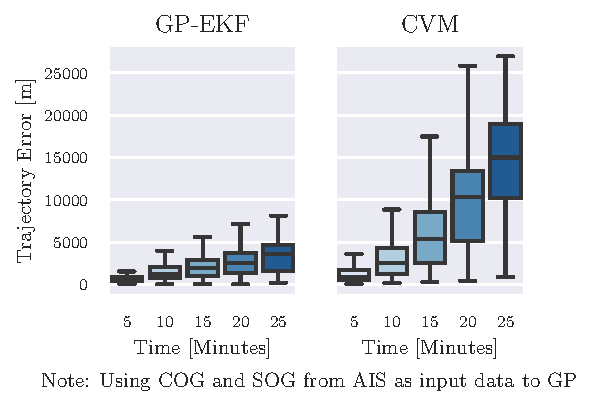
\includegraphics{figures/curved_line_stats/gp_vs_cvm_2.pdf}
    \caption{GP-EKF compared to the CVM method on curved trajectories. As expected, the \acrshort{cvm} yields large trajectory errors on curved trajectories. The GP-EKF performs consistently better, with lower median error as well as lower spread.}
    \label{fig:stats_curved_gp_ekf_cvm}
\end{figure}
As expected, the CVM method struggles with curved trajectories, leading to large trajectory errors. The GP-EKF approach performs significantly better, with overall lower spread and median trajectory error as depicted in \cref{fig:stats_curved_gp_ekf_cvm}.

\section{Effect of the PDAF update}
\begin{figure}[h]
    \centering
    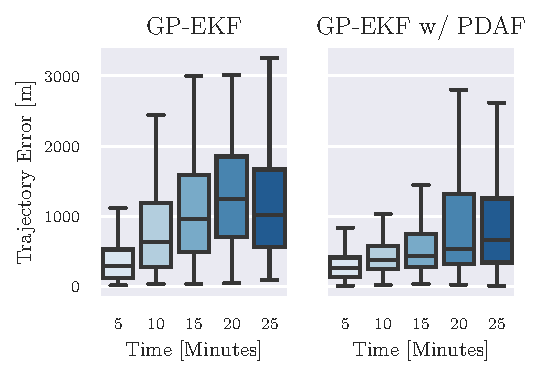
\includegraphics{figures/curved_line_stats/gp_vs_pdaf.pdf}
    \caption{GP-EKF with and without PDAF on curved trajectories for $350$ trajectories. While there are some slight differences, the \acrshort{pdaf} does not appear to have any considerable effect on the trajectory errors.}
    \label{fig:stats_curved_gp_ekf_with_or_without_pdaf}
\end{figure}

\section{Finite Difference vs COG/SOG from AIS}
A key design choice for the GP-EKF is which data source to use for training. The model can either be trained using the \acrshort{cog} and \acrshort{sog} values contained in the \acrshort{ais} samples, or by calculating numerical derivatives of the position through a finite-differences approach. Comparing trajectory error for both approaches on the same test set favors the finite-differences approach, as seen in \cref{fig:stats_curved_gp_ekf_fd_vs_cog}. The finite differences approach performs consistently better, with lower median error and less spread. However, by ignoring the time component, looking back at the path errors in \cref{table:stats_curved_trajectory_path_err} supports the opposite, where the path error is lower for the \acrshort{cog}/\acrshort{sog} approach. This may indicate that the issue is due to inprecise velocity estimates from the \acrshort{sog}, while using the course from the \acrshort{cog} works well.
\begin{figure}[h]
    \centering
    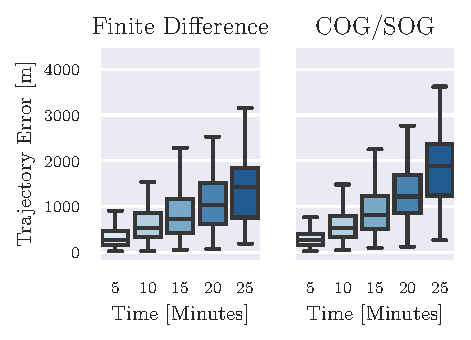
\includegraphics{figures/curved_line_stats/gp_cog_vs_fd.pdf}
    \caption{GP-EKF using finite differences and the \acrshort{cog} and \acrshort{sog} from the AIS dataset on $350$ trajectories. The finite differences approach performs consistently better, with lower median error and spread.}
    \label{fig:stats_curved_gp_ekf_fd_vs_cog}
\end{figure}




\section{Consistency}
Insert plot of NEES here


